\section{Experiments}
\label{sec:exp}

We ask two questions. First, can the gradient-free learner actually
recover a useful weighting when factors are confounded
(\cref{sec:exp:synth})? Second --- the headline --- does a learned
multi-factor value retain gold evidence better than single-factor
baselines on a \emph{real} long-horizon benchmark, once we evaluate
forgetting honestly (\cref{sec:exp:blind})? Both experiments are
CPU-only and use no API calls; embeddings come from a local
sentence-transformer \citep{reimers2019sbert}.

\subsection{Synthetic confound study: does the learner work?}
\label{sec:exp:synth}

\paragraph{Design.}
Each synthetic case contains $4$ gold items and $16$ distractors. Gold
items are \emph{old} but carry the true signal (high goal relevance,
task utility, reliability); distractors are \emph{recent} and carry two
deliberately planted confounds (high value alignment and self relevance)
plus high emotional noise. A policy that trusts all factors equally is
misled by the confounds; a recency- or emotion-only policy keeps the
distractors. We learn $\wvec$ on $60$ training cases to maximise
gold retention at keep-fraction $\keepfrac=0.4$, and report retention on
$60$ disjoint test cases.

\paragraph{Result.}
\Cref{tab:synth} shows that the learner recovers a weighting that retains
\emph{all} gold ($1.00$) on held-out cases, while uniform weighting ---
which trusts the confounds equally --- retains only $0.62$, and
the emotion-, self-, and recency-only policies we test retain $0.00$
(they rank the recent, emotionally noisy distractors first). The learned
weights place the largest mass on the true-signal factors (reliability
$1.36$, task utility $0.88$, goal relevance $0.49$) and drive the
\emph{value-alignment} confound down to $0.09$; the self-relevance
confound is \emph{not} fully suppressed ($1.01$), but the true-signal mass
alone suffices to separate gold from distractors. This is a sanity check,
not the central claim: it shows only that the seven-dimensional black-box
search can fit a \emph{separating mixture} where uniform weighting --- and
the single-factor policies we test --- cannot. We do not test goal-,
task-, or reliability-only baselines on the synthetic case; the real-data
study below tests all four live single factors directly.

\begin{table}[ht!]
\centering\small
\caption{Synthetic confound study: gold retention on $60$ held-out cases
(keep $40\%$). Gold is signalled by goal/task/reliability; distractors
carry planted value-alignment and self-relevance confounds.}
\label{tab:synth}
\begin{tabular}{lr}
\toprule
Policy & Gold retention \\
\midrule
\textbf{learned\_V} & $\mathbf{1.00}$ \\
uniform\_V          & $0.62$ \\
emotion\_only       & $0.00$ \\
self\_only          & $0.00$ \\
recency\_only       & $0.00$ \\
\bottomrule
\end{tabular}
\end{table}

\subsection{Real LongMemEval: blind vs.\ oracle forgetting}
\label{sec:exp:blind}

\paragraph{Setup.}
We use LongMemEval-S \citep{wu2025longmemeval}: questions over long
multi-session chat histories ($\sim\!500$ turns per case) with
gold-evidence turns flagged inside a haystack of distractor sessions. Of
the $500$ questions, $479$ carry at least one flagged gold turn; we use
all $479$. For each case we annotate every turn with the four API-free
factors (emotional intensity, goal relevance, self/user relevance,
reliability; \cref{tab:factors}), rank turns by $V(m)$, keep the top
$\keepfrac=30\%$, and measure the fraction of flagged gold turns
retained. Weights are learned over the live factors on a training split
and evaluated on a disjoint test split; we report mean $\pm$ standard
deviation over $20$ resampled $50/50$ splits ($240$ test cases per rep),
and confirm significance with a per-case bootstrap below. This isolates
the budgeted keep/drop (retention) decision: we do not run an answerer or
the full encode/forget/retrieve loop here, and we report gold-evidence
retention rather than QA accuracy (\cref{sec:limitations}). To pre-compute
the factor annotations once and reuse them across all configurations, we
cache the per-turn factors; every number below is API-free and reproduces
on a single CPU.

\paragraph{The oracle/blind distinction.}
Gold in LongMemEval is defined relative to the evaluation question, so
the \emph{goal-relevance} factor can be computed two ways:
\begin{itemize}[leftmargin=1.4em,itemsep=1pt,topsep=2pt]
\item \textbf{Oracle:} $\mathbf{e}_{\text{goal}}$ is the embedding of the
held-out evaluation question. This peeks at the future query --- a
\emph{retrieval} signal, unavailable when the agent actually forgets.
\item \textbf{Blind:} $\mathbf{e}_{\text{goal}}$ is the centroid of the
ongoing session's user turns (``what is this session about''), the
information genuinely available at consolidation time.
\end{itemize}
All other factors are identical across regimes; only the goal anchor
moves. This is exactly the difference between measuring retrieval and
measuring forgetting.

\paragraph{Result.}
\Cref{tab:blind} and \cref{fig:blind} report both regimes. In the \textbf{oracle} regime,
goal relevance alone retains $0.979$ of gold and the learned value reaches
$0.993$ (uniform $0.939$) --- all near the ceiling: once you can score
similarity to the question, similarity is all you need, and there is no
room for a multi-factor advantage. This is the honest negative that a
query-defined retention metric produces, and it is why such metrics
cannot, by themselves, evaluate a forgetting policy.

In the realistic \textbf{blind} regime the ordering inverts.
Goal-relevance-to-session collapses to $0.286$ (near the $0.30$ chance
floor), emotion to $0.201$, recency to $0.368$, reliability to $0.497$,
and self-relevance --- the strongest single factor --- to $0.518$: no
single cue identifies the future needle without the question. The
\emph{learned multi-factor value} retains $\mathbf{0.770\pm0.011}$,
beating uniform weighting ($0.657$), the best single factor (self,
$0.518$), and recency ($0.368$). A per-case bootstrap ($B{=}10^3$,
resampling the $479$ cases) puts the paired gaps at $+0.120$ vs.\ uniform
($95\%$ CI $[0.091,0.149]$), $+0.402$ vs.\ recency ($[0.350,0.452]$), and
$+0.277$ vs.\ reliability-only ($[0.235,0.319]$); every interval excludes
zero, and the learned policy wins on all $20$ resampled splits.
Multi-factor value's advantage is thus precisely where it should be: in
the query-agnostic forgetting decision, not in query-defined retrieval.

\begin{figure}[ht!]
\centering
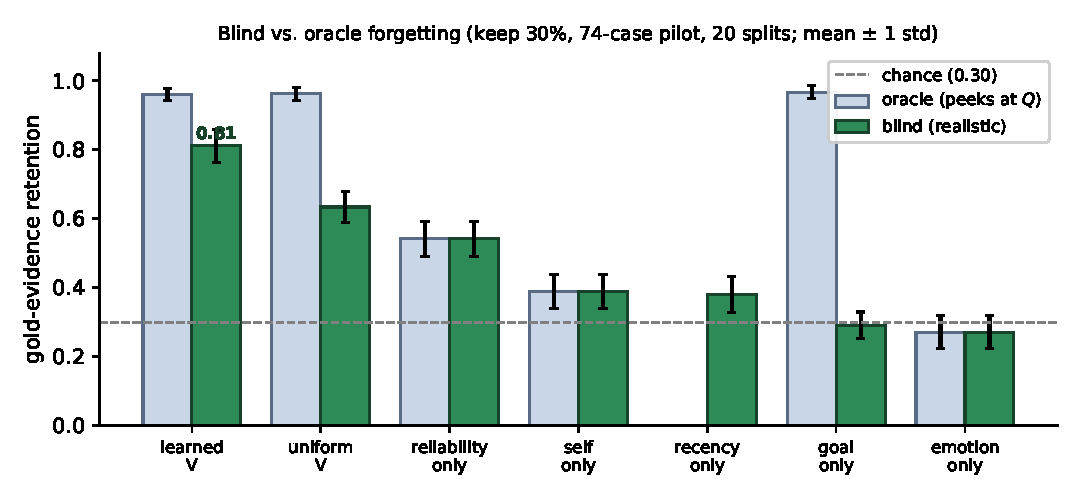
\includegraphics[width=0.82\linewidth]{figures/fig_blind_oracle.pdf}
\caption{\textbf{Blind vs.\ oracle gold retention} (keep $30\%$; all $479$
usable LongMemEval-S cases; $20$ resampled splits, mean $\pm 1$ std). Under
the \emph{oracle} goal anchor (cosine to the held-out question), similarity
alone saturates retention --- a retrieval ceiling. Under the realistic
\emph{blind} anchor (session topic only), every single-factor and recency
baseline collapses toward the chance floor, while the learned multi-factor
value retains $0.77$. Recency has no oracle variant.}
\label{fig:blind}
\end{figure}

\begin{table}[ht!]
\centering\small
\caption{LongMemEval gold retention (keep $30\%$; all $479$ usable cases;
mean $\pm$ std over $20$ resampled test splits, $240$ cases each).
\emph{Oracle} scores goal relevance against the held-out question
(retrieval ceiling); \emph{blind} scores it against the session topic
(realistic forgetting). Self-, emotion-, and reliability-only are
regime-invariant by construction (only the goal anchor moves).}
\label{tab:blind}
\begin{tabular}{lcc}
\toprule
Policy & Oracle (peeks at $Q$) & Blind (realistic) \\
\midrule
\textbf{learned\_V}  & $0.993 \pm 0.005$ & $\mathbf{0.770 \pm 0.011}$ \\
uniform\_V           & $0.939 \pm 0.011$ & $0.657 \pm 0.011$ \\
self\_only           & $0.518 \pm 0.017$ & $0.518 \pm 0.017$ \\
reliability\_only    & $0.497 \pm 0.020$ & $0.497 \pm 0.020$ \\
goal\_only           & $0.979 \pm 0.006$ & $0.286 \pm 0.021$ \\
emotion\_only        & $0.201 \pm 0.017$ & $0.201 \pm 0.017$ \\
recency\_only        & ---               & $0.368 \pm 0.021$ \\
random (keep $30\%$) & ---               & $0.300$ \\
\bottomrule
\end{tabular}
\end{table}

\paragraph{Learned weights are interpretable.}
The mean learned blind weights are reliability $0.64$, emotional
intensity $0.55$, self/user relevance $0.23$, and goal relevance $0.00$.
The policy discovered, from retention alone, that LongMemEval gold is
dominated by \emph{reliable, user-stated, often self-relevant} facts ---
and that session-topic similarity (the blind goal anchor) is useless for
predicting the future needle, so it is driven to zero. This is the
value-directed signal a recency or similarity policy structurally cannot
represent, and it accounts for the $+0.11$ to $+0.40$ retention gap.

\paragraph{Does a neural value help? A nonlinear ablation.}
Our value is linear by design (\cref{sec:method:value}); a natural worry
is that it leaves performance on the table by ignoring factor
interactions (e.g.\ emotion mattering only for self-relevant turns). We
test this directly: we replace the linear value with a small MLP
$g_\theta$ over the same four live factors ($[16,16]$ hidden units),
trained by a pairwise logistic ranking loss (gold ranked above non-gold
within each case), and evaluate it under the identical blind protocol.
The MLP retains $0.773\pm0.011$ versus the linear model's
$0.770\pm0.011$ --- a paired difference of $+0.003\pm0.013$, winning on
only $55\%$ of splits, i.e.\ a statistical tie. On these seven factors the
nonlinear capacity buys nothing: the factors combine near-additively, so
the interpretable linear model is not a compromise but the right choice.
The MLP is an ablation, not a replacement.

\paragraph{The advantage is not budget-specific.}
\Cref{fig:keepfrac} sweeps the keep fraction $\keepfrac \in
\{0.1,\dots,0.5\}$. The learned value leads at every realistic forgetting
budget ($\keepfrac \le 0.4$); only at $\keepfrac{=}0.5$ --- a near-trivial
$50\%$ keep, where all factor-based policies saturate at $0.87$--$0.90$
--- does the best single factor draw level. The multi-factor advantage is
thus largest exactly where forgetting is aggressive and the decision
matters most.

\begin{figure}[ht!]
\centering
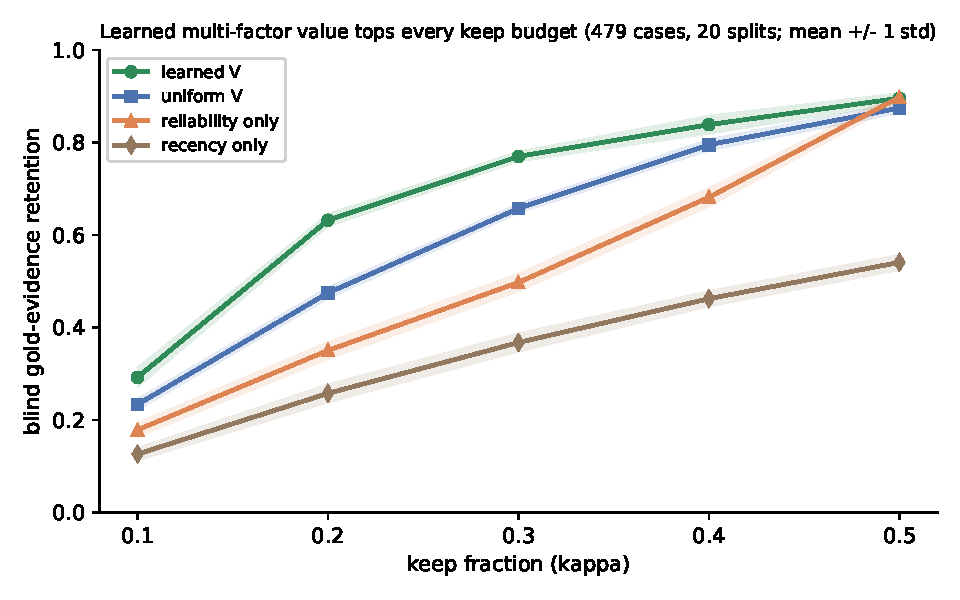
\includegraphics[width=0.74\linewidth]{figures/fig_keepfrac.pdf}
\caption{\textbf{Keep-fraction sweep} (blind regime, $479$ cases, $20$
splits, mean $\pm 1$ std). The learned multi-factor value dominates uniform,
reliability-only, and recency at every aggressive budget
($\keepfrac \le 0.4$); the gap closes only at the near-trivial
$\keepfrac{=}0.5$ where the benchmark saturates.}
\label{fig:keepfrac}
\end{figure}
